\documentclass[12pt, a4paper, oneside]{book}

%%%%%%%%%%%%%%%%%%%%%%%%%%%%%%%%%%%%%%%%%%%%%%%%%%%%%%%%
% 														%
%  					 Basic formatting 					%
% 														%
%%%%%%%%%%%%%%%%%%%%%%%%%%%%%%%%%%%%%%%%%%%%%%%%%%%%%%%%

% Page margins
\usepackage[top=2.5cm, bottom=2.5cm, right=2cm, left=3.5cm]{geometry}

% Line height
\linespread{1.5}

% !!! optional !!!  no hyphenation
\tolerance=100000000
\hyphenpenalty 10000000
\exhyphenpenalty 10000000

% Insert pdf
\usepackage{pdfpages}

% Charset
\usepackage[utf8]{inputenc}
\usepackage[T1]{fontenc}

% Common packages (math fonts, floats etc.)
\usepackage{amsthm}
\usepackage{amsmath}
\usepackage{amsfonts}
\usepackage{amssymb}
\usepackage{float}
\usepackage{array}
\usepackage{pdflscape}
\usepackage{calc}
\usepackage[linesnumbered, ruled]{algorithm2e}
\usepackage{caption}
\usepackage{tikz}
\usepackage{graphicx}
\usepackage{comment}
\usepackage{subcaption}
\usepackage{booktabs}
\usepackage{adjustbox}

%%%%%%%%%%%%%%%%%%%%%%%%%%%%%%%%%%%%%%%%%%%%%%%%%%%%%%%%
% 													 %
%  					Optional formatting 				 %
% 													 %
%%%%%%%%%%%%%%%%%%%%%%%%%%%%%%%%%%%%%%%%%%%%%%%%%%%%%%%%

% Theorems
\theoremstyle{plain}
\newtheorem{theorem}{Theorem}[chapter]
\newtheorem{lemma}[theorem]{Lemma}
\newtheorem{proposition}[theorem]{Proposition}
\newtheorem{corollary}[theorem]{Corollary}

% Definitions and examples
\theoremstyle{definition}
\newtheorem{definition}[theorem]{Definition}
\newtheorem{example}[theorem]{Example}

% Remarks
\theoremstyle{remark}
\newtheorem{remark}[theorem]{Remark}

% !!! optional !!!  Basic caption formatting
\theoremstyle{definition}
%\newtheorem{definition}{Definition}[chapter]

\usepackage{caption}
\captionsetup[figure]{labelfont=bf}
\captionsetup[table]{labelfont=bf}


% !!! optional !!! package for drawing graphs
\usepackage{pgfplots}
\pgfplotsset{width=14cm, height=10cm, compat=1.9}


% !!! optional !!! package for displaying a code
\usepackage{listings}
\definecolor{dkgreen}{rgb}{0,0.6,0}
\definecolor{gray}{rgb}{0.8,0.8,0.7}
\definecolor{myteal}{rgb}{0.17,0.57,0.69}
\definecolor{whitish}{rgb}{0.99, 0.99, 0.98}
\definecolor{mauve}{rgb}{0.58,0,0.82} % used by \lstset (was undefined)

\lstset{frame=tb,
  backgroundcolor=\color{whitish},
  language=C++,
  aboveskip=3mm,
  belowskip=0mm,
  showstringspaces=false,
  columns=flexible,
  basicstyle={\footnotesize\ttfamily},
  numbers=none,
  numberstyle=\tiny\color{gray},
  keywordstyle=\color{blue},
  commentstyle=\color{dkgreen},
  stringstyle=\color{mauve},
  breaklines=true,
  breakatwhitespace=true,
  tabsize=3,  
  emph={int,char,double,float,unsigned,void,bool,MyMesh, VertexIter, VertexVertexCCWIter, std, vector, VertexHandle, vec, AngleOf, max, min} ,
  emphstyle={\color{teal}},
  captionpos=b,
  frame=single,	
  rulecolor=\color{gray}
}
\renewcommand{\lstlistingname}{Code excerpt}
\captionsetup[lstlisting]{labelfont=bf}
\renewcommand\lstlistlistingname{Source codes}

% Image, or a framed placeholder while the file does not exist yet.
%   #1 file, #2 width, #3 placeholder height, #4 what the image must show
\newcommand{\thesisimage}[4]{%
  \IfFileExists{#1}{\includegraphics[width=#2]{#1}}{%
    \fbox{\parbox[c][#3][c]{#2}{\centering\footnotesize
      \textbf{Image placeholder}\\[2pt]\texttt{\detokenize{#1}}\\[4pt]#4}}}}


%%%%%%%%%%%%%%%%%%%%%%%%%%%%%%%%%%%%%%%%%%%%%%%%%%%%%%%%
% 														%
%  			 Information about the author 				%
% 														%
%%%%%%%%%%%%%%%%%%%%%%%%%%%%%%%%%%%%%%%%%%%%%%%%%%%%%%%%

\def\skola{Comenius University in Bratislava}  % Name of the university
\def\fakulta{Faculty of Mathematics, Physics and Informatics} % Name of the faculty
\def\autor{Lucia Držková} % Name of the author



\begin{document}

% Intro pages are numbered by roman numerals
\pagenumbering{roman}

% The good practice is to use separate .tex file for each chapter of the thesis which is placed in the same directory as the main.tex file

%%%%%%%%%%%%%%%%%%%%%%%%%%%%%%%%%%%%%%%%%%%%%%%%%%%%%%%%
% 														%
%  			 			Front page						%
% 														%
%%%%%%%%%%%%%%%%%%%%%%%%%%%%%%%%%%%%%%%%%%%%%%%%%%%%%%%%

% Change the parts with !!!

\thispagestyle{empty} % no numbering

\begin{center}
\textsc{\Large \skola} \\ % include the name of the university and faculty
\bigskip
\textsc{\Large \fakulta}
\end{center}

\vspace{9cm}
\begin{center}
\textbf{\Huge Singularity-aware isosurface extraction}\\  % !!! The name of the thesis 
\bigskip
\Large Master's thesis % The classification of the thesis
\end{center}

\vfill
\textbf{2027 \hfill \autor}  % !!! The year, when the thesis is submitted

\newpage

%%%%%%%%%%%%%%%%%%%%%%%%%%%%%%%%%%%%%%%%%%%%%%%%%%%%%%%%
% 														%
%  			 			Title page						%
% 														%
%%%%%%%%%%%%%%%%%%%%%%%%%%%%%%%%%%%%%%%%%%%%%%%%%%%%%%%%

% it is basically same as the front page, but with additional information

\thispagestyle{empty}
\begin{center}
\textsc{\Large \skola} \\
\bigskip
\textsc{\Large \fakulta}
\end{center}

\vspace{9cm}
\begin{center}
\textbf{\Huge Singularity-aware isosurface extraction}\\ % !!! The name of the thesis 
\bigskip
\Large Master's thesis
\end{center}

\vfill

Study programme:  \textbf{Computer Graphics \& Geometry } \\
\indent  Study field: \hspace{1.1cm} \textbf{Mathematics} \\   \indent Supervisor: \hspace{1.15cm}  \textbf{Mgr. Marcel Makovník, PhD.}\\ % !!! The name and the titles of your supervisor
% !!! The code (****) and the name of the study field, please check if it is correct since it may be changed

\bigskip
\textbf{2027 \hfill \autor} % !!! The year, when the thesis is submitted

\newpage

%%%%%%%%%%%%%%%%%%%%%%%%%%%%%%%%%%%%%%%%%%%%%%%%%%%%%%%%
% 														%
%  			 		Thesis assignment					%
% 														%
%%%%%%%%%%%%%%%%%%%%%%%%%%%%%%%%%%%%%%%%%%%%%%%%%%%%%%%%

% You need to include the pdf file of the assignment generated by AiS2. The assignment must not be scanned or signed!!!

% uncomment the following line if you have the needed .pdf file
%\includepdf[pages={1}]{zadanie.pdf}
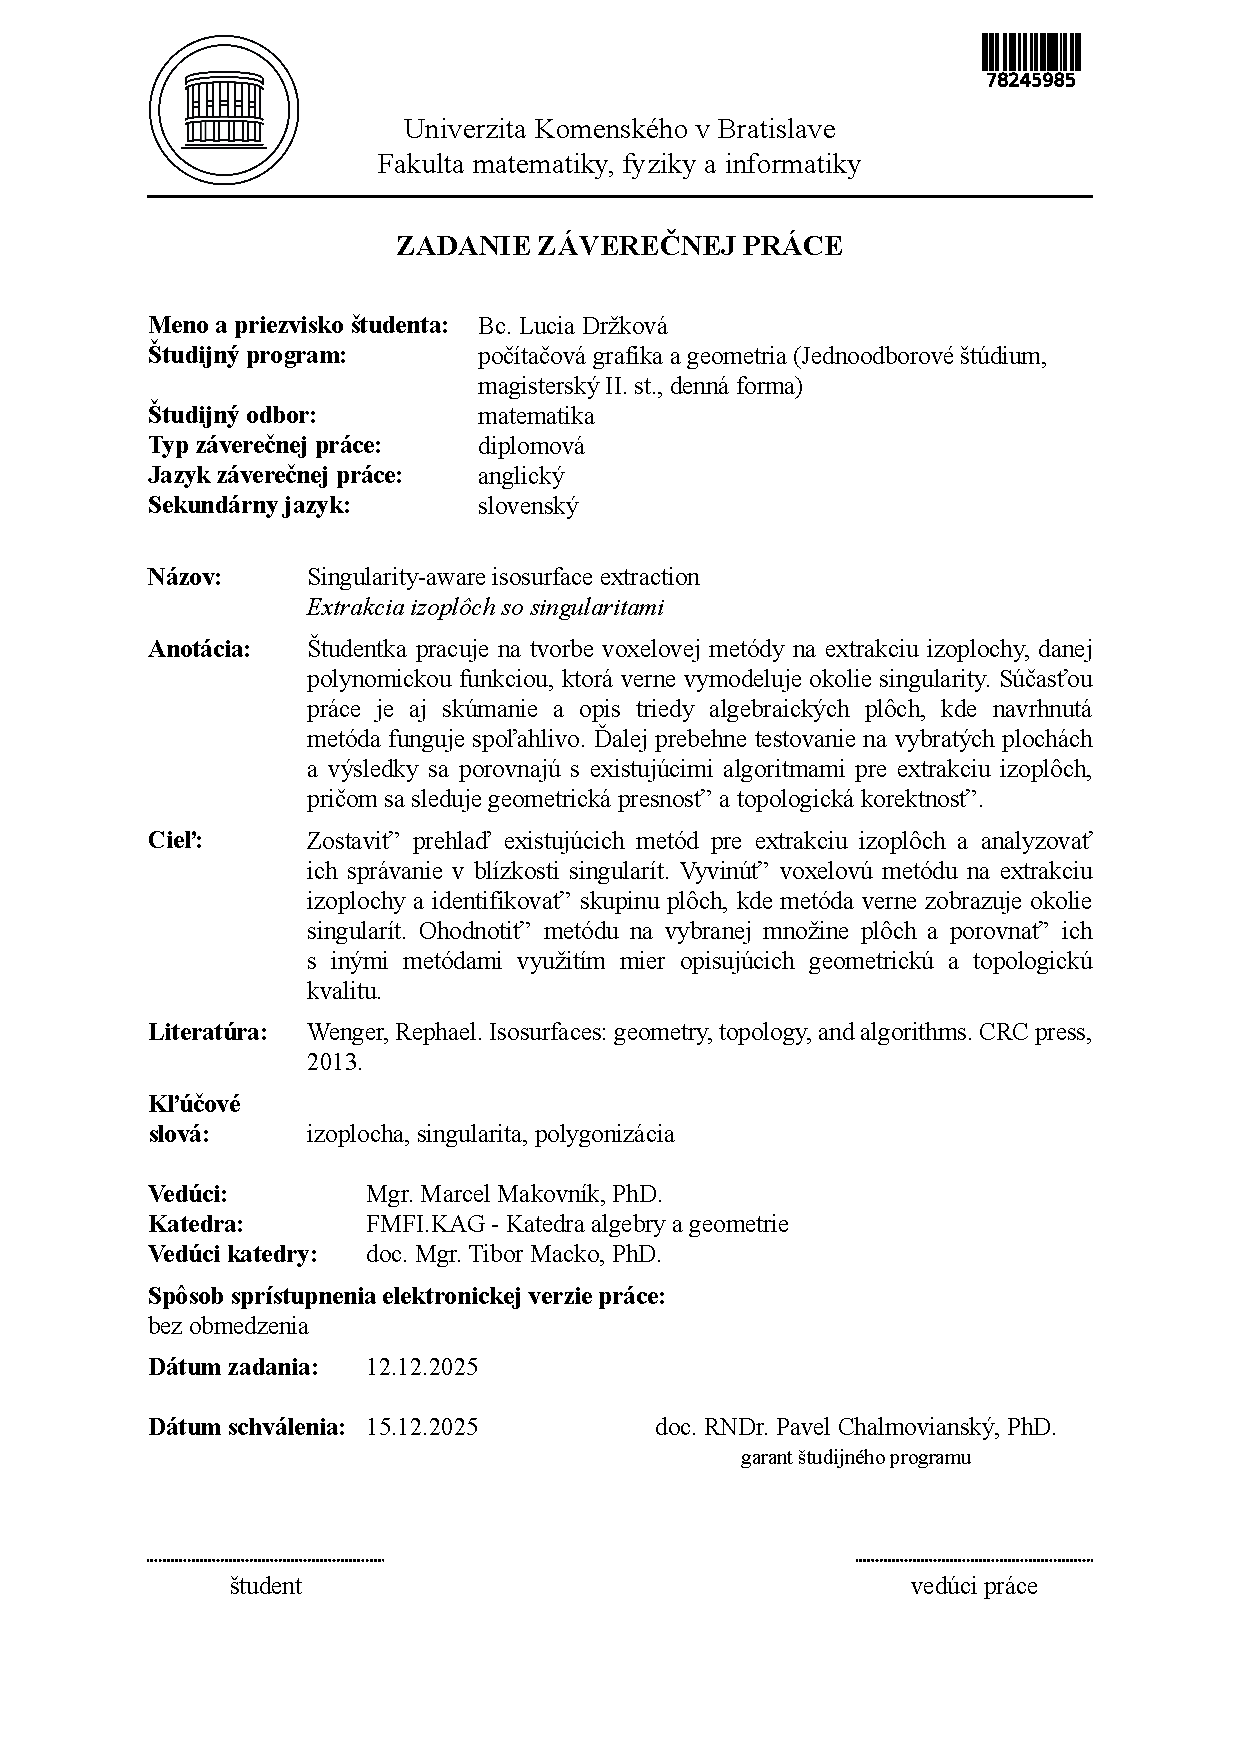
\includepdf[pages={1}]{zadanie-zp_209582.pdf}
 %\includepdf[pages={1}]{Zadanie_eng.pdf}
    
	\begin{titlepage} %čestné prehlásenie
    \section*{Declaration}

		\vspace*{\fill}
		{\setlength{\parindent}{0cm} 
        I hereby declare that I have independently completed the entire Master's thesis on the topic “Singularity-aware isosurface extraction” with the assistance of my supervisor, including all its appendices and illustrations, using only the literature listed in the attached bibliography and artificial intelligence tools. I declare that I have used artificial intelligence tools in accordance with the relevant legal regulations, academic rights and freedoms, ethical and moral principles, while maintaining academic integrity.} \\
		\flushright	........................................\\
	   Lucia Držková	
	\end{titlepage}



%%%%%%%%%%%%%%%%%%%%%%%%%%%%%%%%%%%%%%%%%%%%%%%%%%%%%%%%
% 														%
%  			 		Acknowledgement						%
% 														%
%%%%%%%%%%%%%%%%%%%%%%%%%%%%%%%%%%%%%%%%%%%%%%%%%%%%%%%%

% !!! OPTIONAL !!!
% However, it is nice gesture to give credit to all those who have helped you :-)
{~}\vfill
\section*{Acknowledgement}


	I want to thank...

\newpage

%%%%%%%%%%%%%%%%%%%%%%%%%%%%%%%%%%%%%%%%%%%%%%%%%%%%%%%%
% 														%
%  			 			Abstracts						%
% 														%
%%%%%%%%%%%%%%%%%%%%%%%%%%%%%%%%%%%%%%%%%%%%%%%%%%%%%%%%

% In english language
\section*{Abstract}
The text of abstract in English. \\

\noindent \textbf{keywords:} isosurface, singularity, polygonization

\newpage

% In slovak (national) language
\section*{Abstrakt}
Text abstraktu v slovenčine. \\

\noindent \textbf{kľúčové slová:} izoplocha, singularita, polygonizácia

\newpage

% All of the following are generated automatically

%%%%%%%%%%%%%%%%%%%%%%%%%%%%%%%%%%%%%%%%%%%%%%%%%%%%%%%%
% 														%
%  					Table of contents					%
% 														%
%%%%%%%%%%%%%%%%%%%%%%%%%%%%%%%%%%%%%%%%%%%%%%%%%%%%%%%%

\tableofcontents

%%%%%%%%%%%%%%%%%%%%%%%%%%%%%%%%%%%%%%%%%%%%%%%%%%%%%%%%
% 														%
%  					List of figures			 			%
% 														%
%%%%%%%%%%%%%%%%%%%%%%%%%%%%%%%%%%%%%%%%%%%%%%%%%%%%%%%%

\listoffigures

%%%%%%%%%%%%%%%%%%%%%%%%%%%%%%%%%%%%%%%%%%%%%%%%%%%%%%%%
% 														%
%  					List of tables			 			%
% 														%
%%%%%%%%%%%%%%%%%%%%%%%%%%%%%%%%%%%%%%%%%%%%%%%%%%%%%%%%

% !!! optional !!!
\listoftables
 
%%%%%%%%%%%%%%%%%%%%%%%%%%%%%%%%%%%%%%%%%%%%%%%%%%%%%%%%
% 														%
%  				List of source codes		 			%
% 														%
%%%%%%%%%%%%%%%%%%%%%%%%%%%%%%%%%%%%%%%%%%%%%%%%%%%%%%%% 
% !!! optional !!!
\lstlistoflistings % First pages -- mandatory !!!
\chapter*{Introduction} 
\addcontentsline{toc}{chapter}{Introduction} % the introduction is not numbered, since we have to add it to the table of contents manually
\pagenumbering{arabic} % starting with this page we use arabic page numbering

% the text of the introduction chapter % Introduction is an unnumbered chapter
\newpage

\chapter{Implicit Surfaces and Singularities}
\label{ch:implicit}


\section{Implicit Surfaces}
Implicit surfaces are defined as the set of points satisfying a scalar equation in three-dimensional space. They are used in computer graphics, geometric modeling, visualization, and numerical processing, and we will show their use in voxel-based methods and isosurface extraction algorithms \cite{bloomenthal2000implicit}.

\begin{definition}
\label{def:implicit-surface}
Let $f : \mathbb{R}^3 \to \mathbb{R}$ be a scalar-valued function. The set
\[
S = \{ p \in \mathbb{R}^3 \mid f(p) = 0 \}
\]
is called an \emph{implicit surface} or \emph{zero set} of the function $f$.
\end{definition}

The function $f$ is commonly referred to as the \emph{implicit surface function}. Beyond
identifying which points lie on the surface, the sign of $f$ classifies every point in
space according to its position relative to the surface:
\[
f(p) < 0 \quad \text{inside the surface},
\]
\[
f(p) > 0 \quad \text{outside the surface},
\]
\[
f(p) = 0 \quad \text{on the surface}.
\]

This classification property is one of the major advantages of implicit representations
over parametric approaches \cite{bloomenthal2000implicit}, as illustrated below.


\begin{figure}
    \centering
    \begin{center}
    \begin{tikzpicture}[scale=1.2, font=\small]
        \useasboundingbox (-3.5,-2) rectangle (3.5,2.5);
        \fill[blue!10] (0,0) circle (1.5);
        \draw[very thick, teal] (0,0) circle (1.5);
        \node[align=center] at (0,0) { $f(x,y,z) < 0$ \\ \scriptsize (Inside) };
        \draw[<-, thick] (1.06, 1.06) -- (2.2, 2) node[right, align=left] {
            $f(x,y,z) = 0$ \\
            \scriptsize (Surface $S$)
        };
        \node[align=center] at (2.5, -1) { $f(x,y,z) > 0$ \\ \scriptsize (Outside) };
    \end{tikzpicture}
    \end{center}
    \caption{Unit sphere with sign regions}
    \label{fig:unit_sphere}
\end{figure}


To see why this representation is useful, it is helpful to compare it with the two other
standard representations of surfaces. An explicit surface is represented as
$z=f(x,y)$, which restricts it to height-field configurations, while a parametric surface
defines each coordinate separately,
\[
x=f_x(s,t), \quad y=f_y(s,t), \quad z=f_z(s,t), \qquad (s,t)\in \text{parameter domain},
\]
giving direct access to points on the surface. Implicit surfaces instead treat all
coordinates symmetrically, which allows more complex geometric structures and naturally
supports merging, blending, and deformation operations \cite{bloomenthal2000implicit}.

A natural question is when an implicit surface can locally be described as a smooth
two-dimensional object. This is answered by the following classical result.

\begin{theorem}
Let $f : \mathbb{R}^3 \to \mathbb{R}$ be continuously differentiable in a neighborhood of
a point $p=(x_0,y_0,z_0)$ with $f(p)=0$. If at least one partial derivative of $f$ is
nonzero at $p$, then locally the surface can be expressed as an explicit function of two
variables.
\end{theorem}

The theorem guarantees local regularity whenever the gradient does not vanish, which
motivates the following distinction.

\begin{definition}
\label{def:regular-singular}
A point $p$ on an implicit surface is called a \emph{regular point} if
$\nabla f(p)\neq 0$. Otherwise, $p$ is called a \emph{singular point}.
\end{definition}

The gradient
\[
\nabla f(x,y,z)=
\left(
\frac{\partial f}{\partial x},
\frac{\partial f}{\partial y},
\frac{\partial f}{\partial z}
\right)
\]
defines the local differential structure of the surface and its normal direction. At
regular points this direction is well-defined and the surface locally resembles a smooth
plane; at singular points this structure may break down entirely, which we discuss in
Section~\ref{sec:singularities}.

The most analytically tractable implicit surfaces are those defined by polynomial
functions.

\begin{definition}
An implicit surface is called an \emph{algebraic surface} if the defining function $f$
is polynomial.
\end{definition}

Algebraic surfaces are especially relevant for singularity analysis, because polynomial
structure allows local geometric behavior to be studied through algebraic methods.

An important practical property of implicit surfaces is their suitability for polygonization and voxel-based processing: since the surface is represented by samples of a scalar field, algorithms such as Marching Cubes or Dual Contouring can reconstruct polygonal approximations directly from volumetric data, which makes implicit representations well suited for scientific visualization, medical imaging, and adaptive
geometric modeling \cite{bloomenthal2000implicit}. This combination of algebraic
structure, differential properties, and numerical flexibility is what makes implicit
surfaces a natural framework for studying singularity-aware isosurface extraction, the
topic to which the rest of this chapter is devoted.

\section{Differential and Algebraic Properties of Implicit Surfaces}

Having introduced implicit surfaces as zero sets of a scalar function
$f:\mathbb{R}^3 \rightarrow \mathbb{R}$, we now examine their differential properties in
more detail, starting with the gradient.

\subsection{Gradient and Normal Vector}

The gradient of $f$ is the primary tool for extracting geometric information from an
implicit surface: it encodes how the scalar field changes in each spatial direction and
points perpendicularly to the level set of $f$.

\begin{definition}%[Implicit Surface Gradient]
Let $f(x,y,z)$ be a differentiable scalar field. The gradient of $f$ is
\[
\nabla f(x,y,z) = \left(\frac{\partial f}{\partial x}, \frac{\partial f}{\partial y},
\frac{\partial f}{\partial z}\right).
\]
\end{definition}

\begin{theorem}%[Surface Normal]
If $\nabla f(p) \neq 0$, then the unit normal vector to the implicit surface at $p$ is
\[
\mathbf{n}(p) = \frac{\nabla f(p)}{\|\nabla f(p)\|}.
\]
\end{theorem}

Recall from Definition~\ref{def:regular-singular} that regular points admit a
well-defined normal direction, whereas singular points may not. We next examine how this
translates into the existence of a tangent plane.

\subsection{Tangent Planes and Local Smoothness}

\begin{definition}%[Tangent Plane]
At a regular point $p_0$ on the implicit surface $f(x,y,z)=0$, the tangent plane is
given by
\[
\nabla f(p_0) \cdot (p - p_0) = 0.
\]
\end{definition}

A non-zero gradient therefore ensures local smoothness, and if $f$ is continuously
differentiable, the implicit surface is locally a smooth 2-manifold
\cite{bloomenthal2000implicit}. Beyond this first-order behavior, second-order
derivatives determine how the surface curves.

\subsection{Curvature and Local Geometric Behavior}

\begin{definition}%[Curvature Behavior]
The curvature of an implicit surface is governed by the second-order derivatives of $f$, and is well-defined when $f$ is twice continuously differentiable and $\nabla f \neq 0$.
\end{definition}

Smooth implicit surfaces are therefore classified as $G^2$ continuous under appropriate regularity conditions \cite{bloomenthal2000implicit}. This regularity breaks down at singular points, where the gradient vanishes; we examine such points in detail in Section~\ref{sec:singularities}. As a first illustration, consider the cone
\[
f(x,y,z) = -x^2 + y^2 + z^2,
\]
whose apex at the origin is a singular point where the gradient vanishes, producing a degenerate geometric structure \cite{bloomenthal2000implicit} (Figure~\ref{fig:cone}).

\begin{figure}[!h]
    \centering
    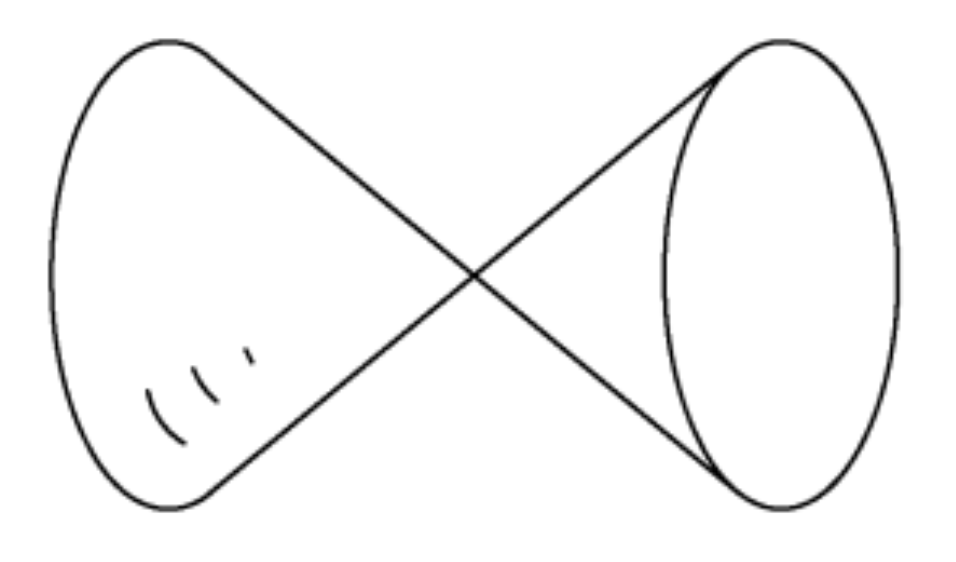
\includegraphics[width=0.4\textwidth]{pictures/cone.png}
    \caption[Cone singularity]{The apex of a cone is a singular point (image retrieved
    from \cite{bloomenthal2000implicit}).}
    \label{fig:cone}
\end{figure}

\subsection{Algebraic Multiplicity and Geometric Behavior}

The algebraic degree of the function $f$ appears to influence the geometry such as the number of intersections with other objects and the local geometry of algebraic surfaces. In general, surfaces with larger degrees will have more complex curvature and singular behaviour. A key relationship between algebraic and geometric structure is that higher algebraic multiplicity at a point may correspond to degeneracies or singularities in the geometry of the surface \cite{bloomenthal2000implicit}.

The following result of this section summarizes the ideas which have been developed on implicit surfaces, leading to a clean sufficient condition for an implicit surface to be a smooth manifold.

% [Manifold Condition]
\begin{theorem}
\label{thm:manifold}
If $f$ is continuously differentiable and $0$ is a regular value of $f$, then the implicit surface $f^{-1}(0)$ is a 2-dimensional manifold embedded in $\mathbb{R}^3$.
\end{theorem}

This result ensures that, under regularity conditions, implicit surfaces behave as smooth geometric objects with well-defined local structure. The following section investigates what happens when this regularity fails.

\section{Singularities of Implicit Surfaces}
\label{sec:singularities}

Recall that a point $p$ on an implicit surface $S=\{p \mid f(p)=0\}$ is \emph{singular} if $\nabla f(p) = 0$ (Definition~\ref{def:regular-singular}). By Theorem~\ref{thm:manifold}, singular points are precisely those where $S$ may fail to be locally manifold-like, since the surface normal and tangent plane are no longer well-defined there. We now study the geometric and numerical consequences of this condition systematically.

\begin{comment}
\subsection{Geometric Interpretation of Singularities}

Geometrically, singularities correspond to locations where the surface loses local flatness, changes topology, or exhibits self-degeneracy, as in the cone example of Figure~\ref{fig:cone}. Such behavior is crucial in both theoretical geometry and numerical computation, as it affects stability in surface reconstruction and rendering algorithms \cite{bloomenthal2000implicit}. These degeneracies occur in several qualitatively distinct forms, which are classified below.


\subsection{Types of Singular Behavior}

These forms are best understood using the singularity theory of smooth mappings, which classifies them via local normal forms \cite{arnold2012singularities}.

\begin{definition}[Types of singular behavior]
The following local forms are commonly encountered:
\begin{itemize}
    \item \textbf{Cusp}: a smooth curve or surface locally forms a pointed tip,
          typically from higher-order degeneracy of derivatives.
    \item \textbf{Swallowtail}: a higher-order singularity with self-intersecting local
          structure and a curvature-sign change in multiple directions.
    \item \textbf{Pinch point}: two local sheets of a surface touch tangentially
          without forming a smooth intersection.
    \item \textbf{Higher-order degeneracy}: not only the first derivative but also
          higher-order derivatives vanish or become linearly dependent, producing
          complex local geometry.
\end{itemize}
\end{definition}

These types can also be distinguished according to whether they affect only a small
neighborhood of a point or the global topology of the surface.

\subsection{Local versus Global Singular Structure}

\begin{itemize}
    \item \textbf{Local singularities} depend only on the behavior of $f$ in an
          infinitesimal neighborhood of a point.
    \item \textbf{Global singularities} affect the topology of the entire surface, such
          as self-intersections or disconnected components.
\end{itemize}

While local singularities determine differential properties, global singular structures
influence the topology and connectivity of the implicit surface. Beyond their theoretical
interest, singularities have direct consequences for numerical methods that reconstruct
implicit surfaces from sampled data.

\subsection{Numerical Difficulties in Polygonization}

Numerical procedures rely on the gradient to estimate normals and classify voxel cells,
and both operations become unreliable when the gradient is close to zero. Near such
points, numerical methods may fail due to unstable normal estimation, ambiguous cell
classification, missed or duplicated surface components, and incorrect topology
reconstruction.

\begin{theorem}[Numerical Instability Near Singularities]
Let $S = \{p \mid f(p)=0\}$ be an implicit surface and let $p_s$ be a singular point such
that $\nabla f(p_s)=0$. Then numerical approximation of the surface normal and local
topology near $p_s$ becomes ill-conditioned.
\end{theorem}

This instability is a fundamental limitation of discrete polygonization methods and
motivates adaptive refinement techniques and alternative implicit evaluation strategies
\cite{bloomenthal2000implicit}.

\subsection*{Summary}

Singularities represent points where the standard manifold structure of an implicit
surface fails, producing both rich geometric phenomena (cusps, swallowtails, pinch
points) and significant numerical challenges. The next two sections address,
respectively, how such singularities can be resolved theoretically, and how they behave
under perturbation; Chapter 2 then turns to how numerical algorithms can be made more
robust in their presence.

\section{Blowup and Resolution of Singularities}

A natural question is whether singularities can be systematically resolved, that is, replaced by a smoother structure capturing the same geometric information without the degeneracy. Consider the context of piecewise smooth dynamical systems. For non-unique singularities such as the visible-invisible two-fold, the non-uniqueness suggests geometric desingularization methods such as regularization and blowup. These ideas are developed systematically in \cite{kristiansen2019resolution}, which combines geometric singular perturbation theory with blowup techniques to resolve non-hyperbolic behavior.

\begin{definition}%[Motivation for desingularization]
Let $X^\pm$ define a piecewise smooth vector field with switching manifold $\Sigma = \{y=0\}$. A singularity $q \in \Sigma$ is called \emph{non-deterministic} if the associated Filippov flow is not uniquely defined at $q$. Desingularization embeds the PWS system into a smooth family $X_\epsilon$ such that the limiting dynamics as $\epsilon \to 0^+$ recover the original system while resolving forward non-uniqueness.
\end{definition}

The central tool is the blowup transformation, which replaces a singular point with a
higher-dimensional manifold capturing directional information of the flow, separating
the different directions from which trajectories can approach it.

\begin{definition}[Blowup in $\mathbb{R}^3$]
Consider a singular point $y=\epsilon=0$. The blowup transformation introduces
polar-type coordinates
\[
(y,\epsilon) = \rho(\bar{y}, \bar{\epsilon}), \quad (\bar{y},\bar{\epsilon}) \in S^1,
\ \rho \geq 0,
\]
where $S^1 = \{(\bar{y},\bar{\epsilon}) \in \mathbb{R}^2 \mid \bar{y}^2 +
\bar{\epsilon}^2 = 1\}$. Under this transformation, the singular point is replaced by the
circle $S^1$, which encodes all possible directional approaches to the singularity.
\end{definition}

\begin{theorem}[Resolution via blowup and regularization \cite{kristiansen2019resolution}]
Let $X_\epsilon$ be a regularized PWS system near a visible--invisible two-fold
singularity $q$. Then, under the blowup transformation and appropriate directional
charts, the system admits a desingularized vector field $X$ on the blown-up space.
Moreover:
\begin{itemize}
    \item The singular two-fold point $q$ lifts to a circle of equilibria
          $\bar{q} \cong S^1$.
    \item The dynamics near $\bar{q}$ separates into invariant directional charts
          corresponding to different asymptotic regimes.
    \item Stable and unstable sliding regions of the original system correspond to
          normally hyperbolic invariant manifolds in the blown-up space.
    \item Loss of hyperbolicity at folds and two-folds becomes a geometric degeneracy
          that can be resolved via local analysis in directional charts.
\end{itemize}
Consequently, forward evolution through the singularity can be uniquely extended in the
regularized system.
\end{theorem}

To work concretely within the blown-up space, one introduces directional charts such as
\[
(y,\epsilon) = (\epsilon \hat{y}, \epsilon) \quad \text{or} \quad (y,\epsilon) =
(y, y \hat{\epsilon}),
\]
which correspond to different regions of the blown-up sphere and allow the desingularized
vector field to be expressed using standard dynamical systems tools. In the
visible--invisible two-fold, for instance, trajectories entering the singularity are
lifted to trajectories on the blown-up circle, where invariant objects such as canards
and sliding flows become separated into distinct geometric objects that can be studied in
a regular setting. In summary, the blowup method shows that singular dynamics in the
original PWS system can be reinterpreted as smooth dynamics on a higher-dimensional
manifold, where local topology is preserved under regularization while the fine structure
of trajectories near the two-fold is governed by invariant manifolds in the blown-up
space \cite{kristiansen2019resolution}.
\end{comment}

\section{Blowup and Resolution of Singularities}
\label{sec:blowup}

The analysis of piecewise smooth (PWS) systems near non-unique singularities, such as the visible–invisible two-fold, requires techniques capable of resolving degeneracies where trajectories lack unique forward evolution. In these systems, trajectories entering a two-fold point are associated with forward non-uniqueness, posing the question of how to continue orbits forward in time. To address this, a combination of regularization and geometric blowup is used to resolve the non-deterministic behavior \cite{kristiansen2019resolution}.

\subsection{Regularization and the Singular System}

Mathematically, a PWS system in $\mathbb{R}^n$ is defined by smooth vector fields $X^+$ and $X^-$ separated by a switching manifold $\Sigma = \{x : y = 0\}$. A regularization is introduced to replace the discontinuous system with a smooth one that recovers the original dynamics as $\epsilon \to 0$:

\begin{equation}
    X_\epsilon(x) = \frac{1}{2}X^+(x)(1 + \phi(\epsilon^{-1}y)) + \frac{1}{2}X^-(x)(1 - \phi(\epsilon^{-1}y)),
\end{equation}

where $\phi$ is a smooth, monotone regularization function. This process introduces a singular point at $\epsilon = 0$, where the vector field is not immediately well-defined in the limit.

\subsection{The Blowup Transformation}

The blowup transformation is a desingularization method that replaces the singular point with a higher-dimensional manifold, such as a circle or sphere, to capture the directional information of the flow. By "blowing up" the point $x=0$, trajectories that were collapsed at the singularity become separated on the new manifold, allowing for a detailed study of their transitions \cite{kristiansen2019resolution}.

\begin{definition}
Given a vector of positive integers $\alpha = (\alpha_1, \dots, \alpha_n)$ called weights, the weighted (or quasihomogeneous) blowup transformation is a mapping $\pi: [0, \infty) \times S^{n-1}_{\alpha} \to \mathbb{R}^n$ defined by:

\begin{equation}
    (\rho, \bar{x}) \mapsto x = (\rho^{\alpha_1} \bar{x}_1, \dots, \rho^{\alpha_n} \bar{x}_n),
\end{equation}

where $S^{n-1}_{\alpha}$ is the unit $\alpha$-sphere.
\end{definition}

For the visible–invisible two-fold, the transformation blows up the singularity to the unit circle \cite{kristiansen2019resolution}.

\begin{figure}[!h]
    \centering
    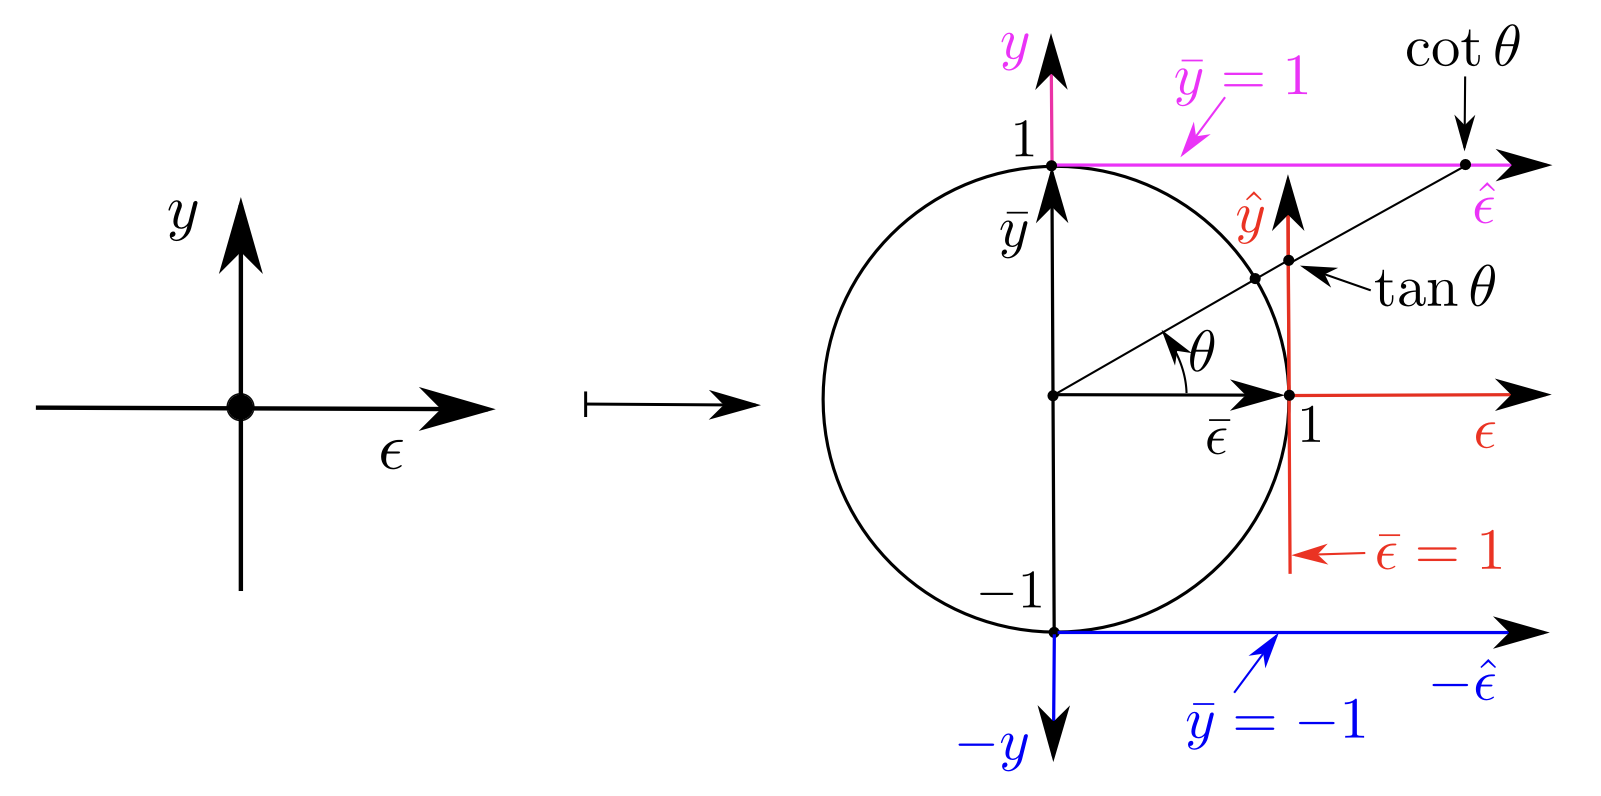
\includegraphics[width=0.6\textwidth]{pictures/blowup.png}
    \caption[Blowup]{Blowup of $y= \epsilon =0$ to the unit circle $y^2+\epsilon^2=1 $. Charts $\epsilon=1$, $y=1$ and $y=-1$ in the blowup transformation (image retrieved
    from \cite{kristiansen2019resolution}).}
    \label{fig:blowup}
\end{figure}


\subsection{Directional Charts and Coordinates}

To analyze the dynamics on the blown-up manifold, the system is expressed in directional charts, which provide an atlas with smooth coordinate changes between overlapping regions. These charts are obtained by setting a specific directional variable to a constant \cite{kristiansen2019resolution}.

\begin{itemize}
    \item \textbf{Chart $K_i^+$:} Defined by the mapping $\bar{x}_i = 1$.
    \item \textbf{Chart $K_i^-$:} Defined by $\bar{x}_i = -1$.
\end{itemize}

These coordinate transformations allow the desingularized vector field to be studied using standard tools of geometric singular perturbation theory.

\subsection{Geometric Resolution and Results}

The main purpose of the process is the determination whether there exist special orbits in the set of possible orbits that have the capacity to evolve further. As far as Kristiansen and Hogan \cite{kristiansen2019resolution} analyze the regularized visible-invisible two-fold, they prove an important technical lemma about the transition through the singular point. Under some conditions, the forward flow of the regularized system possesses a transition map between sections of the phase space that is defined and $C^1$ for all sufficiently small $\epsilon > 0$.

The blowup analysis reveals that there is indeed a unique distinguished forward orbit that characterizes the transition from the two-fold. In this framework, singular dynamics are transformed into smooth dynamics on the higher-dimensional manifold, providing a rigorous geometric foundation for continuing orbits forward in time \cite{kristiansen2019resolution}.

\section{Unfolding and Stability}
\label{sec:unfolding}

The concepts of unfolding and stability are central to understanding how singular structures, such as implicit surfaces or dynamical systems, behave under perturbation. While unfolding in a mathematical sense describes the qualitative changes in a system's behavior near a singularity, structural stability refers to the persistence of its qualitative behavior under small perturbations \cite{ibanez2005shil}.

\subsection{Mathematical Unfolding of Singularities}

An unfolding, in singularity theory and dynamical systems, is a parameterized family of systems which includes a singular (non-structurally stable) one. A system is defined as structurally stable if it lies within the interior of its equivalence class in a topology on a set of dynamical systems. The collection of all non-structurally stable systems is called the bifurcation set \cite{ibanez2005shil}.

For a nilpotent singularity of codimension three in $\mathbb{R}^3$, the vector field $X$ vanishes at the origin with a linear part conjugate to:
\begin{equation}
    J = \begin{pmatrix} 0 & 1 & 0 \\ 0 & 0 & 1 \\ 0 & 0 & 0 \end{pmatrix}.
\end{equation}
Any generic three-parameter unfolding $X_\Lambda$ with parameters $\Lambda = (\lambda_1, \lambda_2, \lambda_3)$ can be expressed in the following normal form:

\begin{equation}
    y \frac{\partial}{\partial x} + z \frac{\partial}{\partial y} + (\lambda + my + nz + x^2 + bxy + cxz + dy^2 + eyz + \alpha(x, y, z, \Lambda)) \frac{\partial}{\partial z},
\end{equation}

where $\alpha$ represents higher-order terms. The parameters $\lambda_i$ allow the system to "unfold," revealing complex behaviors like heteroclinic cycles and Shiľnikov homoclinic orbits that are otherwise hidden at the singularity \cite{ibanez2005shil}.

\begin{comment}
This mathematical sense of unfolding – a family of systems deforming away from a degenerate one – is not unique to dynamical systems. A structurally analogous idea appears in an entirely different field, structural biology, where the same vocabulary of "unfolding" and "stability" is used to describe how a molecule’s three-dimensional configuration responds to applied force. The next subsection draws on this analogy purely for illustration; it does not extend the dynamical-systems theory above but offers a physical intuition for what it means for a stable configuration to be deformed away from equilibrium.

\subsection{Physical and Mechanical Stability}

In physical systems modeled as implicit structures—such as molecular surfaces—stability is often defined by the system's ability to maintain its tertiary structure by minimizing energy and surface exposure \cite{soncini2007mechanical}.

\begin{itemize}
    \item \textbf{Definition of Stability:} Stability is characterized by the interaction of the system (e.g., a polypeptide) with its environment, where the hydrophobic effect is a dominant contributor.
    \item \textbf{Unfolding Process:} A forced unfolding is a dynamic process where a folded configuration is subjected to elongation, causing a progressive loosening of structure. For instance, during the unfolding of alpha-actinin domains, the number of hydrogen bonds ($N_h$) markedly decreases (e.g., from 213 to 68 at 300\% elongation), while the hydrophobic surface available to the solvent increases by approximately 90\%.
\end{itemize}

The magnitude of the force $F(t)$ applied during a mechanical unfolding can be modeled using a harmonic potential:

\begin{equation}
    F(t) = k \cdot [vt - x(t)]
\end{equation}

where $k$ is the spring constant, $v$ is the pulling speed, and $x(t)$ is the coordinate of the system. This energetic perspective complements the mathematical view: while mathematical unfolding describes the topological transitions, mechanical stability describes the resilience of the geometric form against such transitions \cite{ibanez2005shil, soncini2007mechanical}.
\end{comment}

\subsection{Relation to Implicit Surface Reconstruction}

The same ideas apply to implicit surfaces. A surface with a singular point is not structurally stable: an arbitrarily small change of the defining function can remove the singular point, change its type or create new ones, and isosurface extraction algorithms such as Marching Cubes react to exactly such small changes of the sampled scalar field. Embedding the singular surface into a family of perturbed surfaces, an unfolding, makes these changes visible and allows them to be classified \cite{arnold2012singularities,greuel2007introduction}. Chapter~\ref{ch:theory} develops this point of view for one-parameter families $F+kG$.

\begin{comment}
\section{Unfolding and Stability}

While blowup resolves individual singularities, a complementary question is how singular structures behave under perturbation of the system, that is, how they bifurcate as parameters vary. The presentation here follows the framework of generic unfoldings of nilpotent singularities studied in \cite{ibanez2005shil}.

\begin{definition}[Structural stability and bifurcation set]
A vector field $X \in \mathcal{X}$ is structurally stable if there exists a neighbourhood
$U$ of $X$ such that every $Y \in U$ is topologically equivalent to $X$. The bifurcation
set is
\[
B = \{ X \in \mathcal{X} : X \text{ is not structurally stable} \}.
\]
\end{definition}

A central difficulty in dynamical systems is understanding the structure of $B$, even in
low dimensions such as $\mathbb{R}^3$. As discussed in \cite{ibanez2005shil}, one of the
most tractable subsets of $B$ corresponds to vector fields with non-hyperbolic
singularities, which act as organizing centers of bifurcations.

\subsection{Perturbation and stability of singular structures}

A key idea is to study how a singularity behaves when embedded into a parameter family,
formalized by the notion of an unfolding.

\begin{definition}[Unfolding]
Let $X_0$ be a vector field with a singularity at the origin. A $k$-parameter unfolding
of $X_0$ is a family $X_\lambda$, $\lambda \in \mathbb{R}^k$, such that
$X_0 = X_{\lambda=0}$ and $X_\lambda$ depends smoothly on $\lambda$.
\end{definition}

In \cite{ibanez2005shil}, generic unfoldings of the nilpotent singularity of codimension
three in $\mathbb{R}^3$ are shown to generate rich bifurcation structures, including
homoclinic and heteroclinic dynamics.

\begin{definition}[Nilpotent singularity of codimension three]
A vector field near the origin in $\mathbb{R}^3$ has a nilpotent singularity of
codimension three if its linear part is nilpotent and, after a suitable change of
coordinates, it can be written as
\[
y\frac{\partial}{\partial x} + z\frac{\partial}{\partial y} + \left( ax^2 + bxy + cxz +
dy^2 + \cdots \right)\frac{\partial}{\partial z},
\]
with $a \neq 0$ ensuring codimension three behavior.
\end{definition}

Although the main object of study in \cite{ibanez2005shil} is this non-hyperbolic
nilpotent singularity, nearby hyperbolic equilibria play a crucial role in the unfolding,
particularly in the creation of heteroclinic cycles.

\begin{definition}[Stable and unstable manifolds]
Let $p$ be a hyperbolic equilibrium of a vector field $X$. The stable manifold $W^s(p)$
is the set of points whose forward orbits converge to $p$, while the unstable manifold
$W^u(p)$ consists of points whose backward orbits converge to $p$.
\end{definition}

\subsection{Unfolding as local deformation analysis}

In the case studied in \cite{ibanez2005shil}, a generic 3-parameter unfolding of the
nilpotent singularity produces systems of the form
\[
\dot{x} = y, \quad
\dot{y} = z, \quad
\dot{z} = l + my + nz + x^2 + \cdots,
\]
where $(l,m,n)$ are unfolding parameters. As these vary, the dynamics changes
qualitatively, and one of the most striking consequences is the emergence of chaotic
behavior via Shilnikov-type dynamics.

\begin{theorem}[Existence of Shilnikov configurations in unfoldings \cite{ibanez2005shil}]
Any generic unfolding of the nilpotent singularity of codimension three in $\mathbb{R}^3$
contains parameter values for which the system exhibits Shilnikov-type dynamics. In
particular, such unfoldings contain heteroclinic cycles that break to produce Shilnikov
homoclinic orbits.
\end{theorem}

For a critical parameter value, the system exhibits a heteroclinic cycle connecting two
saddle-type equilibria; when the parameters are perturbed, this cycle breaks and gives
rise to homoclinic orbits of Shilnikov type, leading to chaotic dynamics and infinitely
many horseshoes in arbitrarily small neighbourhoods \cite{ibanez2005shil}. This shows that
Shilnikov dynamics is not exceptional but structurally embedded in the unfolding of
sufficiently degenerate singularities: such qualitative phenomena persist under small
parameter perturbations, which explains their robustness in numerical simulations, even
though individual connecting orbits may be destroyed under perturbation. Unfoldings thus
serve as a bridge between local singularity theory and global dynamical complexity: the
geometry of invariant manifolds under unfolding fully determines the emergence of complex
dynamics such as Shilnikov homoclinic orbits \cite{ibanez2005shil}.
\end{comment}


\chapter{Numerical Isosurface Extraction}
\label{ch:extraction}
\section{Voxel Grids and Scalar Fields}

A \emph{scalar field} is a function that assigns a scalar value to every point in a domain, typically $\mathbb{R}^3 \rightarrow \mathbb{R}$. In the context of isosurface extraction, the surface is implicitly defined as the set of points where the scalar field attains a constant value (iso-value), a representation fundamental to implicit modeling and surface extraction techniques \cite{bloomenthal1997introduction}.

\begin{definition}
    %\textbf{(Scalar Field Representation)}
Let $f:\mathbb{R}^3 \rightarrow \mathbb{R}$ be a continuous function. An isosurface $\mathcal{S}$ corresponding to an iso-value $c \in \mathbb{R}$ is
\[
\mathcal{S} = \{ \mathbf{x} \in \mathbb{R}^3 \mid f(\mathbf{x}) = c \}.
\]
\end{definition}

This formulation underlies voxel-based representations used in surface extraction algorithms \cite{bloomenthal1997introduction,lorensen1998marching}. In practice, continuous scalar fields must be discretized for computation using a \emph{voxel grid}, where space is partitioned into a uniform lattice of cubic cells whose vertices store sampled values of the scalar field. The classical \emph{Marching Cubes} algorithm introduced a structured approach for evaluating scalar fields at grid vertices and reconstructing surfaces within each voxel \cite{lorensen1998marching}.

\begin{definition}
    %\textbf{(Uniform Voxel Grid)}
\textbf{A uniform voxel grid} partitions a bounded domain $\Omega \subset \mathbb{R}^3$ into
equally sized cubes of side length $h$, where each vertex stores a sampled scalar value $f(\mathbf{x}_i)$.
\end{definition}

To reconstruct the scalar field at points other than grid vertices, the most common method is \emph{trilinear interpolation}, which linearly interpolates values along each axis.

\begin{theorem}
    %\textbf{(Trilinear Interpolation Continuity)}
Let $f$ be sampled at the eight corners of a voxel. The trilinear interpolation function $f_h(\mathbf{x})$ is continuous inside the voxel and piecewise linear along each axis.
\end{theorem}

\begin{example}
    Given voxel corner values $f_{000}, \dots, f_{111}$, the interpolated value at
    $(x,y,z)$ is
\[
f_h(x,y,z) = \sum_{i,j,k \in \{0,1\}} f_{ijk}(1-x)^{1-i}x^i(1-y)^{1-j}y^j
(1-z)^{1-k}z^k.
\]
\end{example}

This scheme form the basis of techniques used in isosurface extraction algorithms such as Marching Cubes \cite{lorensen1998marching}. However, the use of uniform grids is not efficient when there is large variation in the scalar field across the domain. Adaptive approaches involves refinement of the grid only where required. The concept of Adaptively Sampled Distance Fields is one such technique that employs hierarchical refinement of voxels depending on their variation in the scalar field \cite{frisken2000adaptively}.

\begin{definition}
    %\textbf{(Adaptive Voxel Grid)}
\textbf{An adaptive voxel grid} is a hierarchical decomposition of $\Omega$ into voxels of varying sizes, refined according to a local error criterion.
\end{definition}

Frisken et al.\ show that adaptive sampling significantly reduces memory usage without compromising on surface quality since refinement is done only at places of curvature or sharp changes in the scalar field \cite{frisken2000adaptively}.

However, another problem faced is due to the limited precision of floating point arithmetic. When evaluating scalar fields near singularities or regions of high curvature, small numerical errors may lead to incorrect sign evaluation of $f(\mathbf{x}) - c$: if two nearby evaluations satisfy $f(\mathbf{x}) \approx c \pm \epsilon$, rounding errors may incorrectly classify voxel corners as inside or outside the surface, leading to topological inconsistencies in the extracted mesh. Goldberg emphasizes that floating-point arithmetic is not associative and can introduce significant rounding errors in geometric computations \cite{goldberg1991every}; such issues are particularly critical in isosurface extraction, where sign changes determine topology. Together, adaptive sampling and careful numerical treatment are what allow voxel grids to serve as a stable computational foundation for the isosurface extraction algorithms developed in the remainder of this chapter. 
%\cite{lorensen1998marching,bloomenthal1997introduction,frisken2000adaptively,cignoni1998metro,goldberg1991every}.

\section{Marching Cubes}
\label{sec:marching-cubes}

The Marching Cubes algorithm is a classical method for extracting a polygonal approximation of an isosurface from a discretized scalar field. Expanding on the concept of a voxel grid from the last section, cells are classified based on whether their vertices lie above or below the isosurface defined by the values of the scalar field in those vertices, followed by choosing a predetermined triangulation that represents the isosurface in the cell. The original formulation by Lorensen and Cline introduced a systematic way to convert volumetric scalar data into triangle meshes \cite{lorensen1998marching}.

\begin{definition}
    %\textbf{(Cell Classification)}
Let a voxel cell have eight vertices $v_0, \dots, v_7$, each with scalar value
$f(v_i)$. Given an iso-value $c$, each vertex is classified as
\[
\text{inside} \quad \text{if } f(v_i) \geq c, \qquad \text{outside} \quad \text{if }
f(v_i) < c.
\]
\end{definition}

This binary classification induces a bit-pattern (cube index) in $[0,255]$, which uniquely determines the triangulation configuration via a precomputed lookup table
\cite{lorensen1998marching}.
\begin{figure}[!h]
    \centering
        \begin{subfigure}{0.55\textwidth}
        \centering
        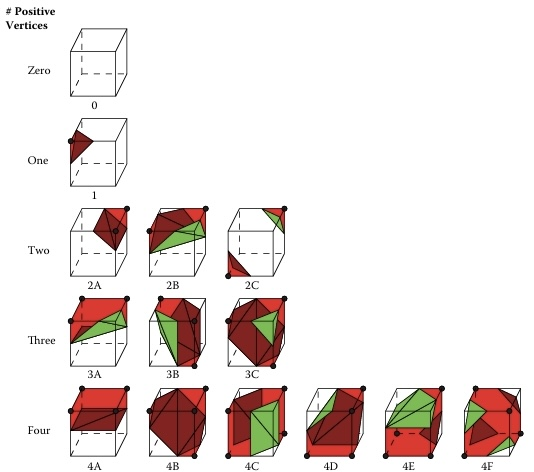
\includegraphics[width=\textwidth]{pictures/marching_cubes1.jpeg}
        \end{subfigure}
    \hspace{0.03\textwidth}
        \begin{subfigure}{0.35\textwidth}
        \centering
        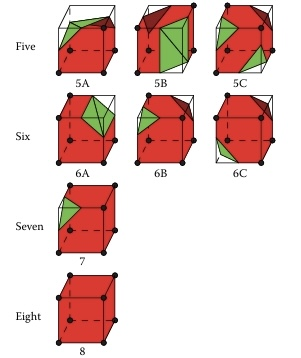
\includegraphics[width=\textwidth]{pictures/marching_cubes2.jpeg}
        \end{subfigure}
    \caption[Cube configurations]{Positive red regions contain positive black vertices and represent areas where the scalar value is above the isovalue. Green surfaces indicate the visible portion of the extracted isosurface, while dark red surfaces represent parts of the isosurface that are hidde behind the positive red regions in the 3D view (image retrieved from \cite{wenger2013}).}
\label{fig:marching_cubes}
\end{figure}

\subsection{Edge Interpolation}

Once the intersected edges of a voxel are identified through cell classification, the algorithm determines the precise coordinates where the isosurface crosses the grid. Because the scalar field is only sampled at discrete vertices, the exact intersection point must be approximated. Following the principles of piecewise-linear continuation, the Marching Cubes algorithm assumes that the scalar field $f$ varies linearly along each edge of the cube.

If the scalar values at two adjacent vertices $v_a$ and $v_b$ lie on opposite sides of the isovalue $c$, there exists at least one point $\mathbf{p}$ on the segment $v_a v_b$ such that $f(\mathbf{p}) = c$.

\begin{definition}%[Edge Intersection Point]
\label{def:edge-interp}
For an edge connecting vertices $v_a$ and $v_b$, with associated scalar values $s_a$ and $s_b$ and isovalue $\sigma$, the point $\mathbf{p}$ is defined as:
\begin{equation}
p = (1 - \alpha) v_a + \alpha v_b, \quad \text{where} \quad \alpha = \frac{\sigma - s_a}{s_b - s_a}.
\end{equation}
The parameter $\alpha \in [0, 1]$ represents the normalized distance along the edge. This linear approximation is computationally efficient and ensures that the reconstructed mesh remains continuous across adjacent voxels.
\end{definition}

The mathematical validity of this interpolation depends on the structural stability of the scalar field near the edge. If the gradient $\nabla f$ is non-zero (a regular point), the surface is locally a differentiable manifold, and the linear approximation provides a first-order accurate reconstruction. Near a singular point this assumption fails. On an edge with a sign change the denominator $s_b - s_a$ cannot vanish, since $|s_b-s_a|=|s_a|+|s_b|$, but both values are small because the gradient is close to zero, so their relative rounding errors are large, and the field along the edge is far from linear because the higher-order terms dominate. The interpolated vertex position is therefore unreliable. This is precisely the kind of sensitivity to small perturbations used in Unfolding, a singular point in the scalar field sits on the boundary of a bifurcation set, so an arbitrarily small change in the sampled values can push the local configuration across it, producing a qualitatively different (and possibly incorrect) triangulation. Such regions therefore typically require higher-order interpolation or adaptive refinement to recover the correct local topology \cite{frisken2000adaptively}.

\subsection{Ambiguities and Topological Inconsistencies}

A well-known limitation of the original Marching Cubes algorithm is that the same cube configuration can yield multiple valid triangulations. For instance, a face with alternating inside/outside vertices admits two valid diagonal connections, and choosing the wrong one may result in a non-manifold surface. This happens because the triangulation is determined locally within each cell without any consistency check against adjacent cells (see Figure~\ref{fig:ambiguity_comparison}).

%Dürst first identified such topological inconsistencies and showed that naive triangulation may violate surface continuity constraints \cite{durst1988marching}. To resolve such ambiguities, Nielson and Hamann proposed the \emph{Asymptotic Decider}, which uses bilinear interpolation over cube faces to consistently determine topology \cite{nielson1991asymptotic}.

\begin{figure}[!h]
    \centering
    \begin{subfigure}{0.48\textwidth}
        \centering
        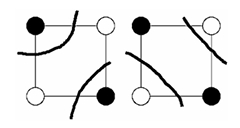
\includegraphics[width=\textwidth]{pictures/ambiguity.jpeg}
        \caption{Ambiguous face configuration (image retrieved from \cite{brentzen2012})}
        \label{fig:ambiguity2}
    \end{subfigure}
    \hfill
    \begin{subfigure}{0.48\textwidth}
        \centering
        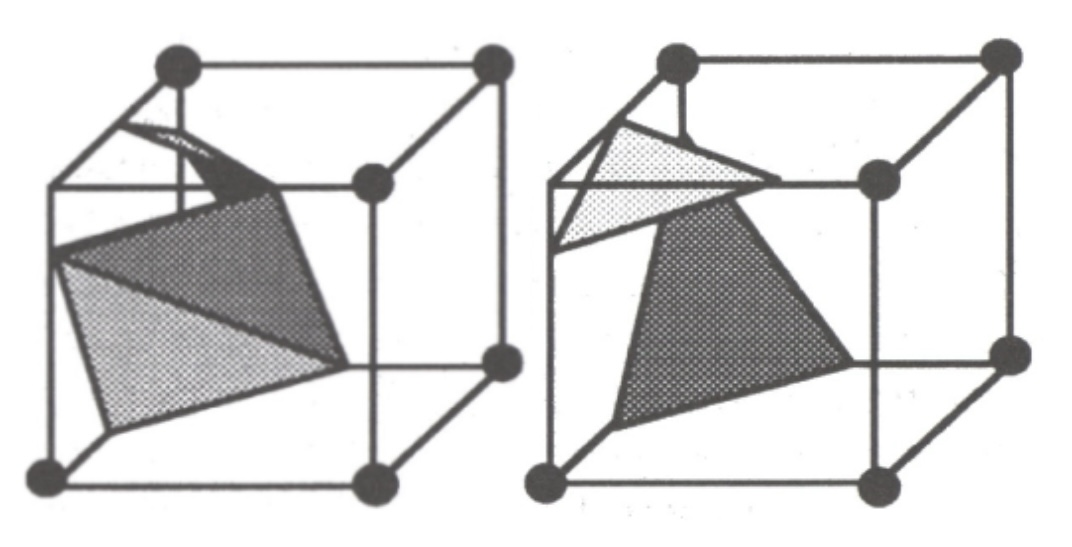
\includegraphics[width=\textwidth]{pictures/ambiguity3.jpeg}
        \caption{Two possible triangulations that yield a topologically correct isovalue surface (image retrieved from \cite{nielson1991asymptotic}).}
        \label{fig:ambiguity3}
    \end{subfigure}
    \caption{Comparison of ambiguities in 2D and 3D.}
    \label{fig:ambiguity_comparison}
\end{figure}

\begin{comment}
\begin{definition}
    \textbf{(Asymptotic Decider)}
Given bilinearly interpolated scalar values on a cube face, the decision of how to
connect edges is based on evaluating the saddle point of the interpolation function.
\end{definition}

Chernyaev further extended the algorithm with \emph{Marching Cubes 33}, which introduces
a more complete case table and resolves remaining ambiguities by refining cube
subdivision rules \cite{chernyaev1995marching}.

\subsection{Topological Correctness Improvements}

Lewiner et al.\ later proposed an efficient reformulation of Marching Cubes that
guarantees consistent topology by systematically resolving ambiguous cases
\cite{lewiner2003efficient}.

\begin{theorem}
    \textbf{(Topological Consistency Guarantee)}
Under the refined case classification scheme of Lewiner et al., the resulting mesh is
guaranteed to be free of cracks and topological inconsistencies for regular scalar
fields.
\end{theorem}

Despite these improvements, Marching Cubes can still fail near singular points where the
gradient is undefined or highly unstable: small perturbations in vertex values can lead
to different triangulations, causing visual artifacts or incorrect topology, especially
where the scalar field changes rapidly or is poorly sampled
\cite{lorensen1998marching,lewiner2003efficient}. Marching Cubes nonetheless remains
foundational; the Asymptotic Decider and Marching Cubes 33 significantly improve its
robustness and topological guarantees
\cite{lorensen1998marching,nielson1991asymptotic,chernyaev1995mc33,lewiner2003mc}.
\end{comment}

\section{Marching Tetrahedra}

The ambiguity issues in Marching Cubes are directly related to the hexahedral nature of the grid cells of this algorithm, which allows for several possible triangulations in certain configurations. The Marching Tetrahedra algorithms eliminates such ambiguities.

A voxel is split into a set of disjoint tetrahedra, each consisting of four vertices selected among the eight cube vertices, thereby partitioning the original cell into tetrahedra. For a tetrahedron $t$ with vertices $v_0, v_1, v_2, v_3$ and scalar values $s_i$, an isosurface is extracted by linearly interpolating along edges where the scalar function crosses zero relative to an iso-value $c$.

Since a tetrahedron has only four vertices, the amount of the possible sign configurations becomes much smaller as compared to the 256 cases in Marching Cubes. Each tetrahedron can be triangulated using one of the at most 16 possible sign configurations (see Figure~\ref{fig:marching_tetrahedra}).

\begin{figure}[!h]
    \centering
    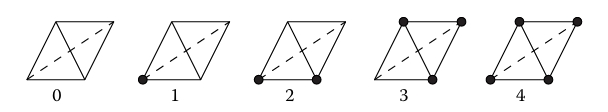
\includegraphics[width=0.8\textwidth]{pictures/marching_tetrahedra.jpeg}
    \caption[Tetrahedra configurations]{Tetrahedra configurations (image retrieved from \cite{wenger2013})} 
    \label{fig:marching_tetrahedra}
\end{figure} 

The intersection points of the edges of a tetrahedron are found using the same interpolation formula from Definition~\ref{def:edge-interp}, now applied to the edges of a tetrahedron instead of the cube edges.


Marching Tetrahedra guarantees that no face ambiguity occurs within a single simplex, ensuring locally consistent topology under correct interpolation assumptions. In other words, this method does not produce face-based ambiguity issues, like those seen in Marching Cubes. The drawback of this is that tetrahedral techniques sacrifice geometric efficiency for topological robustness. In Marching Cubes, one cube may create up to 5 triangles in each case, whereas its tetrahedral decomposition results in creation of a larger number of triangles because of multiple simplex interpolations, but all these tetrahedrons ensure creation of consistent triangulations \cite{nielson2008dual}.

Despite this robustness, the increased number of generated primitives can lead to generation of denser meshes in comparison with Marching Cubes, and inconsistent global triangulation may still happen if neighboring cubes use different subdivision schemes. Overall, Marching Tetrahedra sacrifices geometric simplicity for the sake of topological robustness in ambiguous and numerically difficult situations.

\section{Dual Contouring}

In both Marching Cubes and Marching Tetrahedra algorithms, the surface vertices lie along the grid edges and are determined through interpolation, which fails to represent sharp geometric features like edges or corners due to the nature of interpolation smoothing. The method introduced by Ju et al. \cite{ju2002dual} named Dual Contouring deals with this issue by changing the process to optimization-based placement of the surface vertices, meaning that the surface vertex is placed not on the grid edge, but inside the cell where the gradient field of the scalar field changes sign, using the geometric energy minimization function based on the local geometry of the surface.

For the regular voxel grid, the dual grid has one vertex per grid cell, not one per grid corner; each dual vertex corresponds to a local approximation of the isosurface in the corresponding cell. The data used to position each dual vertex is captured by Hermite data.

\begin{definition}
    \textbf{Hermite Data} is a set of samples associated with grid edges where the isosurface is intersected, consisting of intersection points $\mathbf{p}_i$, surface normals $\mathbf{n}_i$, and optionally gradient estimates of the scalar field.
\end{definition}

These values provide both positional and differential information crucial for accurate reconstruction. The edge intersection points themselves are computed using the same linear interpolation formula as in Marching Cubes (Definition~\ref{def:edge-interp}), but unlike Marching Cubes, Dual Contouring does not place vertices directly at these points; instead, it uses them as constraints in an optimization problem.

\subsection{Quadratic Error Function (QEF)}

The optimization problem to find the position of each dual vertex is based on the Quadratic Error Function that computes the point in the cell that best satisfies all local tangent plane constraints simultaneously.

\begin{definition}
\textbf{(QEF)}
Given Hermite constraints $(\mathbf{p}_i, \mathbf{n}_i)$, the QEF is
\[
E(\mathbf{x}) = \sum_i \left( \mathbf{n}_i \cdot (\mathbf{x} - \mathbf{p}_i) \right)^2.
\]
\end{definition}

The optimal position of the vertex $\mathbf{x}^* = \arg\min_{\mathbf{x}} E(\mathbf{x})$. The solution $\mathbf{x}^*$ to the QEF minimizes the squared distance to all tangent planes defined by Hermite data. The least-square formulation enables a stable and efficient computation of vertex positions with geometric details \cite{ju2002dual}.  

One of the most important advantages of the Dual Contouring algorithm is its ability to preserve sharp edges and corners, while the Marching Cubes algorithm interpolates these features. Feature-sensitive reconstruction requires explicit handling of discontinuities in the surface normal field, achieved by incorporating Hermite constraints directly into vertex positioning \cite{kobbelt2001feature}.

In regions where Hermite constraints are sparse or poorly conditioned, for instance, when normals are nearly parallel or intersection points nearly collinear, the QEF may become ill-defined. In order to achieve stability in such degenerate cases, it is essential to use regularization techniques like positional constraints or clamping solution \cite{ju2002dual}.  Modern extensions to adaptive grids allow higher resolution only where needed.  Adaptive dual contouring leads to substantial memory savings without compromising on sharp feature retention.

With precise Hermite data, the vertices obtained through QEF minimization will lie very close to the isosurface along with retaining the first order geometry of edges and corners. Dual Contouring technique thus evolves from interpolation based surface extraction to optimization based surface reconstruction technique utilizing Hermite data, enabling superior feature preservation and more flexible topology handling \cite{ju2002dual,kobbelt2001feature}.

\section{Differential Properties in Polygonization}
\begin{comment}
Polygonal isosurface extraction methods aim not only to reconstruct geometry but also to
approximate the differential properties of the underlying implicit surface, namely
surface normals, curvature, and geometric error, all essential for visual fidelity and
numerical correctness.

\begin{definition}
    \textbf{(Surface Normals on Polygonal Meshes)}
Given a triangle mesh $\mathcal{M}$ approximating an isosurface, the normal vector at a
vertex is typically a weighted average of adjacent face normals,
\[
\mathbf{n}_v = \frac{\sum_{f \in \mathcal{N}(v)} w_f \mathbf{n}_f}{\left\|\sum_{f \in
\mathcal{N}(v)} w_f \mathbf{n}_f \right\|},
\]
where $\mathcal{N}(v)$ is the set of adjacent faces and $w_f$ a weighting factor based on
area or angle.
\end{definition}

Rusinkiewicz shows that such averaging schemes give robust normal estimates on discrete
meshes, especially combined with local neighborhood analysis
\cite{rusinkiewicz2004estimating}. Beyond normals, the second-order geometry of the
surface is captured by curvature.

\begin{definition}
    \textbf{(Curvature on Triangle Meshes)}
Curvature describes how a surface deviates from being planar; for a polyhedral surface
it is approximated using discrete differential operators applied to vertex
neighborhoods.
\end{definition}

Taubin introduces a tensor-based formulation of curvature estimation on polygonal
meshes, derived from local variations of normals \cite{taubin1995estimating}.

\begin{theorem}
    \textbf{(Discrete Curvature Approximation)}
Let $\mathcal{M}$ be a sufficiently dense triangulation of a smooth surface. Then the
discrete curvature tensor converges to the continuous curvature tensor as the mesh
resolution increases.
\end{theorem}

\textit{Proof sketch.} Convergence follows from the consistency of local surface
approximations and the stability of weighted normal averaging in shrinking neighborhoods
\cite{taubin1995estimating}.

\subsection{Curvature-Sensitive Reconstruction}

Regions of high curvature typically require finer sampling to preserve geometric detail,
while flatter regions can be approximated with fewer primitives; Rusinkiewicz
demonstrates that curvature estimation can also improve smoothing, remeshing, and feature
detection \cite{rusinkiewicz2004estimating}. Beyond curvature, it is also important to
quantify how closely a polygonal mesh approximates the original surface.

\begin{definition}
    \textbf{(Geometric Error Metrics)}
Let $\mathcal{S}$ be the original implicit surface and $\mathcal{M}$ its polygonal
approximation. The geometric error at $\mathbf{x} \in \mathcal{M}$ is the Euclidean
distance to the closest point on $\mathcal{S}$,
\[
E(\mathbf{x}) = \min_{\mathbf{y} \in \mathcal{S}} \|\mathbf{x} - \mathbf{y}\|.
\]
\end{definition}

Cignoni et al.\ formalize this notion in the Metro framework for measuring deviation
between meshes and reference surfaces \cite{cignoni1998metro}.

\begin{theorem}
    \textbf{(Error Accumulation in Polygonization)}
Let $\mathcal{M}_h$ be a mesh generated with resolution parameter $h$. Then the
geometric error satisfies $E(\mathcal{M}_h) = \mathcal{O}(h)$ under uniform sampling
assumptions.
\end{theorem}

This follows from the relationship between sampling density and approximation accuracy
in surface reconstruction \cite{cignoni1998metro}.

\subsection{Relation to Quadric Error Metrics}

Garland and Heckbert introduced quadric error metrics for measuring and minimizing
geometric deviation during surface simplification; although designed for decimation, the
same quadratic-error idea is closely related to error control in reconstruction.

\begin{definition}
    \textbf{(Quadric Error Metric)}
Each vertex is associated with a quadratic form representing the squared distance to a
set of planes, whose optimal position minimizes $E(\mathbf{x}) = \mathbf{x}^T Q
\mathbf{x}$, where $Q$ is the accumulated error matrix.
\end{definition}

This formulation provides a computationally efficient way to approximate geometric
deviation \cite{garland1997surface}. Beyond geometric accuracy, the topology of the
reconstructed surface must also be correct: it must preserve the right connectivity and
avoid artificial holes or self-intersections. Edelsbrunner and Mücke introduced
$\alpha$-shapes as a formal framework for defining the topology of a point set based on a
scale parameter $\alpha$ \cite{edelsbrunner1994three}.

\begin{theorem}
    \textbf{(Topological Consistency of Alpha Shapes)}
For a sufficiently dense sampling of a compact surface, the $\alpha$-shape converges to
the correct topological structure of the original object for an appropriate choice of
$\alpha$.
\end{theorem}

If a surface is under-sampled in regions of high curvature, however, polygonization may
introduce spurious handles or disconnected components, which alpha-shape theory explains
as incorrect scale selection \cite{edelsbrunner1994three}.

Taken together, normals, curvature, and geometric error provide the essential feedback
for evaluating and improving polygonal isosurface reconstruction, connecting discrete
mesh representations back to the underlying smooth geometry with which this chapter began
\cite{rusinkiewicz2004estimating,taubin1995curvature,cignoni1998metro,garland1997quadric,edelsbrunner1994three}.
\end{comment}




% Use \input{} to insert your own numbered chapters (e.g. Basic notions, Results, Conclusion)
%
% \input{01-basic-notions.tex}
%

\newpage

% after the main part of the thesis and conclusion you include the bibliography, which is stored in the "bibliography.bib" file

\bibliographystyle{alpha} % we use Surname/year format for references, e.g. Boris Delaunay, ..., 1934 = [Del34]
\bibliography{bibliography} % include the reference file

\end{document}
